\hypertarget{role-of-software-architecture}{%
\section{Role of Software
Architect(ure)}\label{role-of-software-architecture}}

\begin{tcolorbox}[colback=blue!5!white,colframe=blue!75!black]
\begin{itemize}
    \item Software Architecture
    \begin{itemize}
        \item Origin of the term; description
        \item Some definitions
        \item Kinds of software architecture
        \item Software architecture and building architecture
        \item Software architecture disciplines
        \item Adequacy of software architecture
        \item Need for and difficulties of a software architecture
    \end{itemize}
    \item Role of software architect
    \begin{itemize}
        \item Software architect’s tasks
    \end{itemize}
\end{itemize}
\end{tcolorbox}

\hypertarget{what-is-software-architecture}{%
\subsection{What is Software
Architecture}\label{what-is-software-architecture}}

A software system's architecture is the set of principal design
decisions about the system. Software architecture is the blueprint for a
software system's construction and evolution.

\begin{itemize}
\tightlist
\item
  Definition of

  \begin{itemize}
  \tightlist
  \item
    Classes, Hirarchies, etc
  \item
    High Levle Abstractions

    \begin{itemize}
    \tightlist
    \item
      Components
    \item
      Relations
    \end{itemize}
  \item
    Decisions
  \end{itemize}
\item
  On basis of

  \begin{itemize}
  \tightlist
  \item
    functional requirements
  \item
    non-functional requirements
  \end{itemize}
\end{itemize}

A software architecture provides an overview and supports an easy
understanding. It describes a solution that fits

\begin{itemize}
\tightlist
\item
  fulfills functional and non-functional requirements
\item
  can be realized (political and organizational)
\item
  can be implemented (e.g.~proof through prototypes)
\end{itemize}

At the end:

\begin{itemize}
\tightlist
\item
  process: design a solution
\item
  product: models, documentation, prototypes
\item
  means: eases implementation of larger system
\end{itemize}

\hypertarget{what-design-decisions}{%
\subsubsection{What Design Decisions}\label{what-design-decisions}}

\begin{itemize}
\tightlist
\item
  Structural
\item
  Behavioral
\item
  Interaction
\item
  Non-functional
\end{itemize}

\hypertarget{definition-of-ieee}{%
\subsubsection{Definition of IEEE}\label{definition-of-ieee}}

Architecture: The fundamental organization of a system embodied in its
components, their relationships to each other, and to the environment,
and the principles guiding its design and evolution.

\hypertarget{kind-of-software-architecture}{%
\subsection{Kind of Software
Architecture}\label{kind-of-software-architecture}}

\begin{itemize}
\tightlist
\item
  Enterprise architecture

  \begin{itemize}
  \tightlist
  \item
    metaphor: city planning
  \end{itemize}
\item
  Application architecture

  \begin{itemize}
  \tightlist
  \item
    metaphor: building architecture
  \end{itemize}
\end{itemize}

Software Architecture vs.~building architecture:

\begin{figure}[H]
\centering
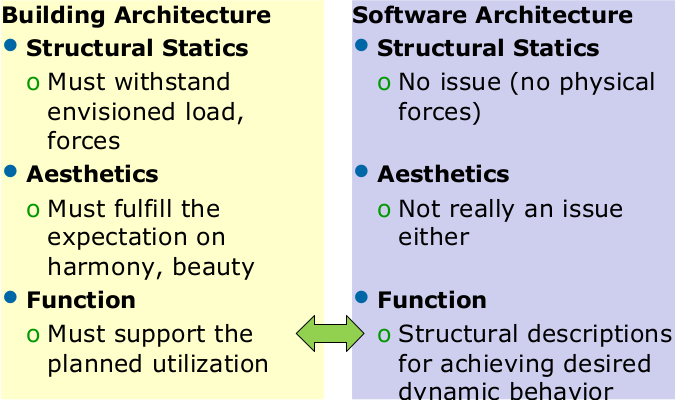
\includegraphics[width=0.5\textwidth]{figures/buildingSoftwareArchitecture.png}
\caption{Building vs.~Software Architecture}
\end{figure}

\hypertarget{proving-the-software-architecture}{%
\subsection{Proving the software
architecture}\label{proving-the-software-architecture}}

We only can prove the software architecture by doing some prototypes of
the hardest componenst and prove that it fulfills the requirements.

\hypertarget{documentation}{%
\subsection{Documentation}\label{documentation}}

Software Architecture is a set of models of the overall software system.
All requirements relevant for the system's construction must be
addressed, e.g.~Extendibility Timing Performance Security.

\hypertarget{architectural-views-kruchten}{%
\subsection{Architectural Views
Kruchten}\label{architectural-views-kruchten}}

Different stakeholders need different information. With different views
on the project, you are able to split the different requirements and
extract the proper information for these stakeholders. Kruchten suggests
4+1 views.

\hypertarget{logical-view}{%
\subsubsection{Logical View}\label{logical-view}}

The logical view is concerned with the functionality that the system
provides to end-users.\\
\textit{Class diagram, Communication diagram, Sequence diagram.}

\hypertarget{development-view}{%
\subsubsection{Development View}\label{development-view}}

The development view illustrates a system from a programmer's
perspective and is concerned with software management. This view is also
known as the implementation view.\\
\textit{Package Diagram, UML Component Diagram}

\hypertarget{process-view}{%
\subsubsection{Process View}\label{process-view}}

The process view deals with the dynamic aspects of the system, explains
the system processes and how they communicate, and focuses on the
runtime behavior of the system.. \\
\textit{Activity diagram}

\hypertarget{physical-view}{%
\subsubsection{Physical View}\label{physical-view}}

The physical view depicts the system from a system engineer's
point-of-view. It is concerned with the topology of software components
on the physical layer, as well as communication between these
components. Also the question where to deploy the system\\
\textit{Deployment diagram}

\hypertarget{scenarios}{%
\subsubsection{(+1)Scenarios}\label{scenarios}}

The description of an architecture is illustrated using a small set of
use cases, or scenarios which become a fifth view.\\
\textit{Use case diagram}

\hypertarget{why-architecture}{%
\subsection{Why architecture}\label{why-architecture}}

\begin{itemize}
\tightlist
\item
  communication among stakeholders

  \begin{itemize}
  \tightlist
  \item
    common understanding about the system
  \item
    get consensus
  \item
    basis for discussions and decisions
  \end{itemize}
\item
  document design decisions

  \begin{itemize}
  \tightlist
  \item
    guidelines for implementation
  \item
    basis for evolution and iterations
  \item
    helps structuring team and planning
  \item
    checkpoints for goal achievement
  \end{itemize}
\item
  abstraction of the system (as built)

  \begin{itemize}
  \tightlist
  \item
    for building product lines and homogeneous systems
  \item
    for outsourcing or acquiring parts
  \end{itemize}
\end{itemize}

\hypertarget{some-typical-misconceptions}{%
\subsection{Some typical
misconceptions}\label{some-typical-misconceptions}}

\begin{itemize}
\tightlist
\item
  Architecture is the same as design

  \begin{itemize}
  \tightlist
  \item
    Architecture is more an overall view and design is a specific
    structure of one component.
  \end{itemize}
\item
  Architecture is about infrastructure

  \begin{itemize}
  \tightlist
  \item
    ``Frameworks, application servers, and databases from a minor part
    of the problem space only''
  \end{itemize}
\item
  Architecture solves technical problems

  \begin{itemize}
  \tightlist
  \item
    ``Chances are your biggest problem isn't technical''
  \end{itemize}
\item
  Architecture is rigid and fixed (up front)

  \begin{itemize}
  \tightlist
  \item
    ``Understand the impact of change''
  \item
    ``Start with a walking skeleton''
  \item
    ``Great software is not built, it is grown''
  \end{itemize}
\item
  Architecture is pure science or pure art

  \begin{itemize}
  \tightlist
  \item
    requires both and more
  \end{itemize}
\end{itemize}

\hypertarget{software-architect}{%
\subsection{Software Architect}\label{software-architect}}

\begin{itemize}
\tightlist
\item
  Decide (under uncertainty, but decide)

  \begin{itemize}
  \tightlist
  \item
    ``Use uncertainty as a driver'', ``Architectural tradeoffs''
  \end{itemize}
\item
  Document (adequately)

  \begin{itemize}
  \tightlist
  \item
    ``Communication is king, clarity and leadership its servants''
  \item
    ``Record your rationale''
  \end{itemize}
\item
  Proof feasibility

  \begin{itemize}
  \tightlist
  \item
    ``One line of working code is worth 500 lines of specification''
  \item
    ``Try before choosing''
  \end{itemize}
\item
  Program

  \begin{itemize}
  \tightlist
  \item
    ``Architects must be hands on''
  \item
    ``Before anything an architect is a developer''
  \item
    ``If you design it, you should be able to code it''
  \item
    J. Coplien: Architect always/also implements
  \end{itemize}
\item
  Communicate

  \begin{itemize}
  \tightlist
  \item
    ``Stand up'', ``Talk the talk''
  \item
    ``Learn a new language''
  \end{itemize}
\item
  Negotiate (with stakeholders)

  \begin{itemize}
  \tightlist
  \item
    ``Seek the value in requested capabilities''
  \item
    ``You're negotiating more than you think''
  \end{itemize}
\item
  Simplify

  \begin{itemize}
  \tightlist
  \item
    ``Simplify essential complexity; reduce accidental complexity''
  \item
    ``Simplicity before generality, use before reuse''
  \item
    ``Make sure the simple stuff is simple''
  \end{itemize}
\item
  Standardize

  \begin{itemize}
  \tightlist
  \item
    ``Reduce the entropy''
  \end{itemize}
\item
  Listen

  \begin{itemize}
  \tightlist
  \item
    ``Hear the stakeholder's concerns''
  \end{itemize}
\item
  Observe

  \begin{itemize}
  \tightlist
  \item
    ``Don't control, but observe''
  \item
    ``Get the 1000-foot view''
  \end{itemize}
\item
  Think (about the future)

  \begin{itemize}
  \tightlist
  \item
    ``Everything will ultimately fail''
  \item
    ``Focus on application support and maintenance''
  \item
    ``Your system is legacy; design for it''
  \item
    ``You can't provide future-proof solutions''
  \end{itemize}
\item
  Lead

  \begin{itemize}
  \tightlist
  \item
    ``Give developers autonomy''
  \item
    ``There is no `I' in architecture''
  \end{itemize}
\end{itemize}

\hypertarget{architects-anti-behavior}{%
\subsubsection{Architect's
Anti-Behavior}\label{architects-anti-behavior}}

\begin{itemize}
\tightlist
\item
  design in an ivory tower
\item
  design by committee
\item
  design by power point
\item
  re-invent the wheel
\item
  over engineering
\item
  under engineering
\item
  premature framework design
\end{itemize}

\hypertarget{top-5-mistakes}{%
\subsubsection{Top 5 mistakes}\label{top-5-mistakes}}

\begin{itemize}
\tightlist
\item
  Believing the requirements
\item
  Being seduced by the technology
\item
  Majoring on your strengths and neglecting other areas
\item
  Not stopping designers from designing
\item
  Thinking you can do it all yourself
\end{itemize}

\clearpage